\documentclass[11pt]{article}
\usepackage{graphicx}
\usepackage{float}
\usepackage{amsmath}
\usepackage{amsfonts}
\usepackage[brazilian]{babel}
\usepackage[utf8]{inputenc}
\usepackage[T1]{fontenc}

\begin{document}

\title{Funções: Exercícios Complementares}
\author{Erik Perillo}
\date{}
\maketitle

\newpage

\section{Exercícios}
\begin{enumerate}
	\item Um cientista descobrou que, a cada árvore de frutinhas que há em uma
		região, há uma média de $23$ morcegos naquele local.
	\begin{enumerate}
		\item Escreva uma função que descreva o número de morcegos de acordo
			com o número de árvores de frutinhas em uma região.
		\item Qual a raiz da função?
		\item Foi descoberta uma região com 34 árvores frutíferas. Quantos 
			morcegos é pra ter nessa região?
		\item Desenhe o gráfico da função.
	\end{enumerate}

	\item Um fazendeiro investiu $450$ reais em uma plantação de tomates e 
		conseguiu colher $1000$ deles. O fazendeiro pretende vender cada tomate
		a $70$ centavos cada.
	\begin{enumerate}
		\item Escreva uma função que descreve o lucro do fazendeiro de acordo
			com quantos tomates ele vende.
		\item Quantos tomates ele tem que vender para não ter prejuízo?
		\item Em qual ponto $y$ a função passa pelo eixo $y$?
		\item Quanto ele vai lucrar se vender todos os tomates?
		\item Desenhe o gráfico da função.
	\end{enumerate}

	\item O dono de um açougue precisa manter as carnes no seu freezer bem 
		frias. Ele não quer usar eletricidade, mas tem bastante gelo à sua 
		disposição. Ele descobriu que, a cada uma tonelada de gelo que ele joga
		na sala, a temperatura dela desce em 20 graus. A temperatura inicial
		da sala, sem gelo algum, é de 30 graus.
	\begin{enumerate}
		\item Escreva uma função que descreve a temperatura da sala de acordo
			com o número de toneladas de gelo na sala.
		\item Quantas toneladas de gelo ele vai precisar para ter a sala a 
			$-18$ graus?
		\item Desenhe o gráfico da função.
	\end{enumerate}

	\item Um astrônomo descobriu que, a cada 8 estrelas que existem em uma
		galáxia, há 128 planetas nela.
	\begin{enumerate}
		\item Escreva uma função que descreve o número de planetas em uma 
			galáxia de acordo com o número de estrelas nela.
		\item Desenhe o gráfico da função.
	\end{enumerate}
\end{enumerate}

\newpage

\begin{enumerate}
	\item 
	\begin{enumerate}
		\item $f(x) = 23x$
		\item $f(x) = 23x = 0 \implies x = 0$
		\item $f(34) = 23*34 = 782$
		\item -- 
			\begin{figure}[H]
				\centering
				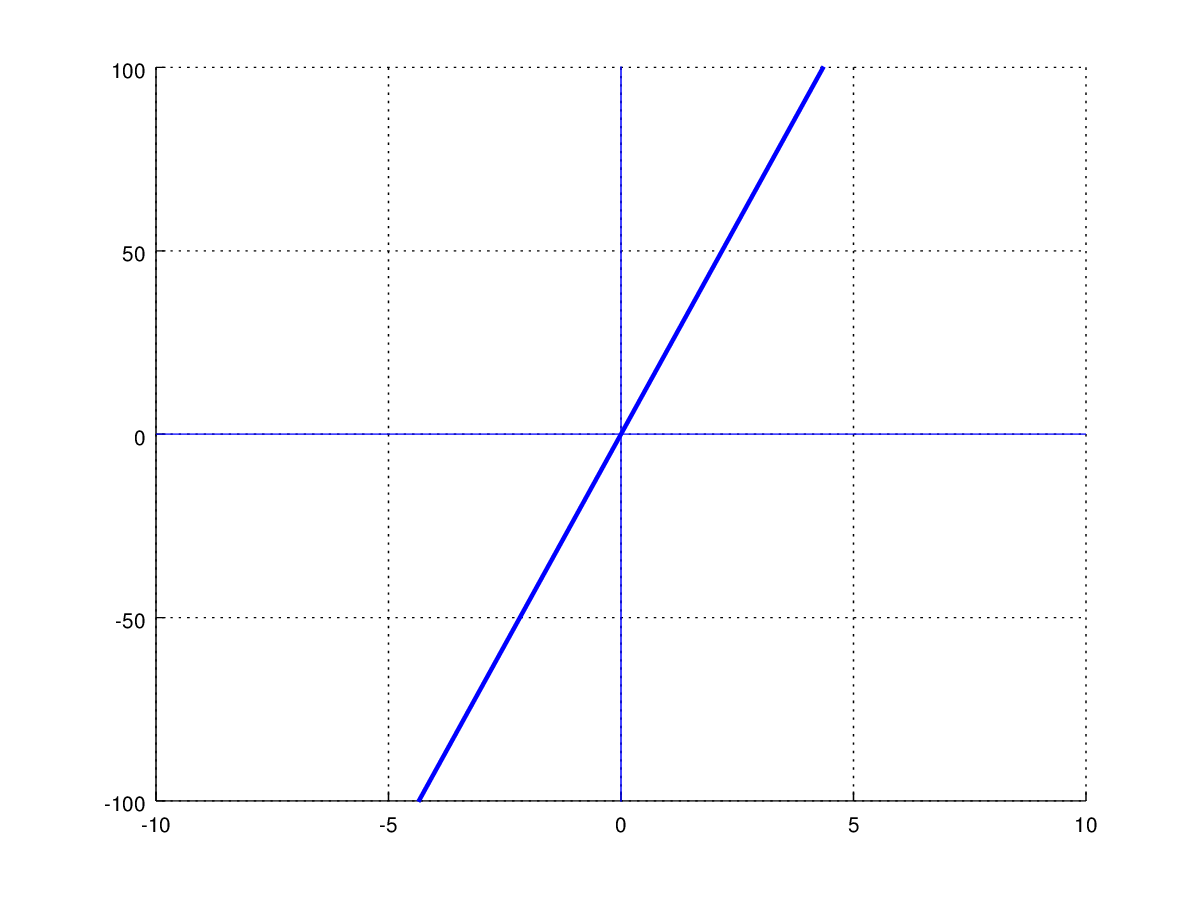
\includegraphics[width=0.9\textwidth]{imgs/ex1c.png}
			\end{figure}
	\end{enumerate}

	\item 
	\begin{enumerate}
		\item $f(x) = 0.7x - 450$ (70 centavos são $0.7$ reais)
		\item $f(x) > 0 \implies 0.7x - 450 > 0 \implies x > 450/0.7 \implies
			x > 642.86$
		\item $f(0) = -450 \implies y = -450$
		\item $f(1000) = 0.7*1000 - 450 = 700 - 450 = 250$
		\item -- 
			\begin{figure}[H]
				\centering
				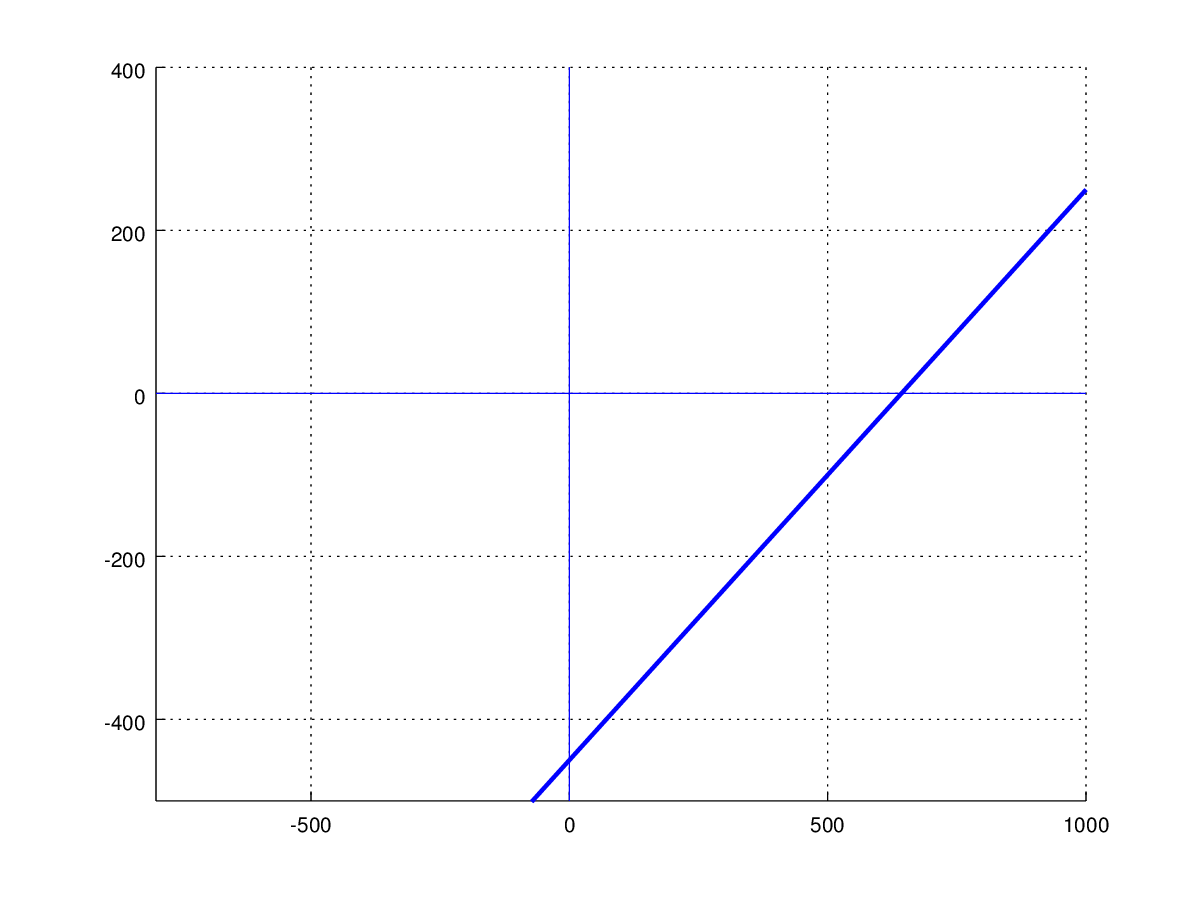
\includegraphics[width=0.9\textwidth]{imgs/ex2c.png}
			\end{figure}
	\end{enumerate}

	\item 
	\begin{enumerate}
		\item $f(x) = 30 - 20x$
		\item $f(x) = -18 = 30 - 20x \implies -20x = -48 \implies x = 
			\frac{-48}{-20} = 2.4$
		\item -- 
			\begin{figure}[H]
				\centering
				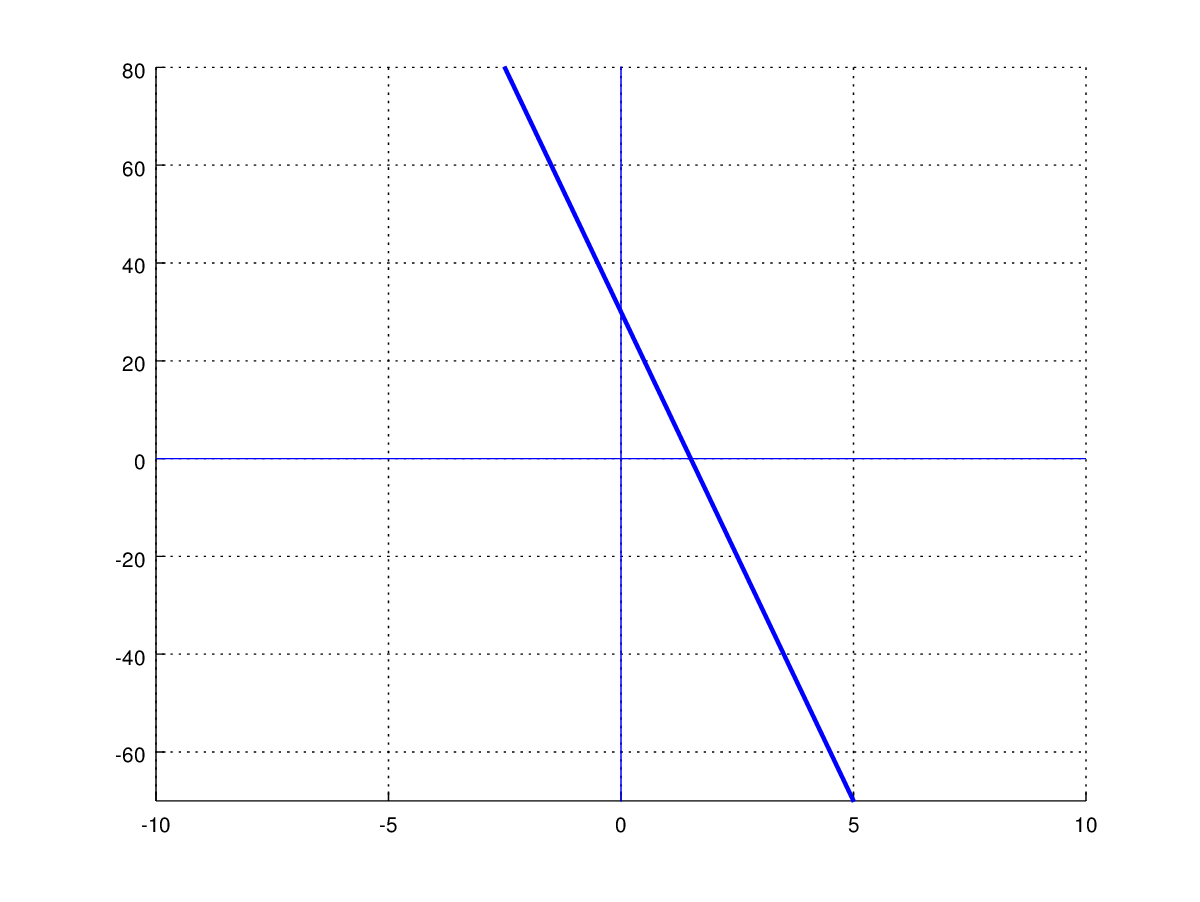
\includegraphics[width=0.9\textwidth]{imgs/ex3c.png}
			\end{figure}
	\end{enumerate}

	\item 
	\begin{enumerate}
		\item Se a cada 8 estrelas há 128 planetas, a cada uma estrelas há um
			oitavo disso, ou seja, $128/8 = 16$ planetas. Assim,
			$$f(x) = 16x$$
		\item -- 
			\begin{figure}[H]
				\centering
				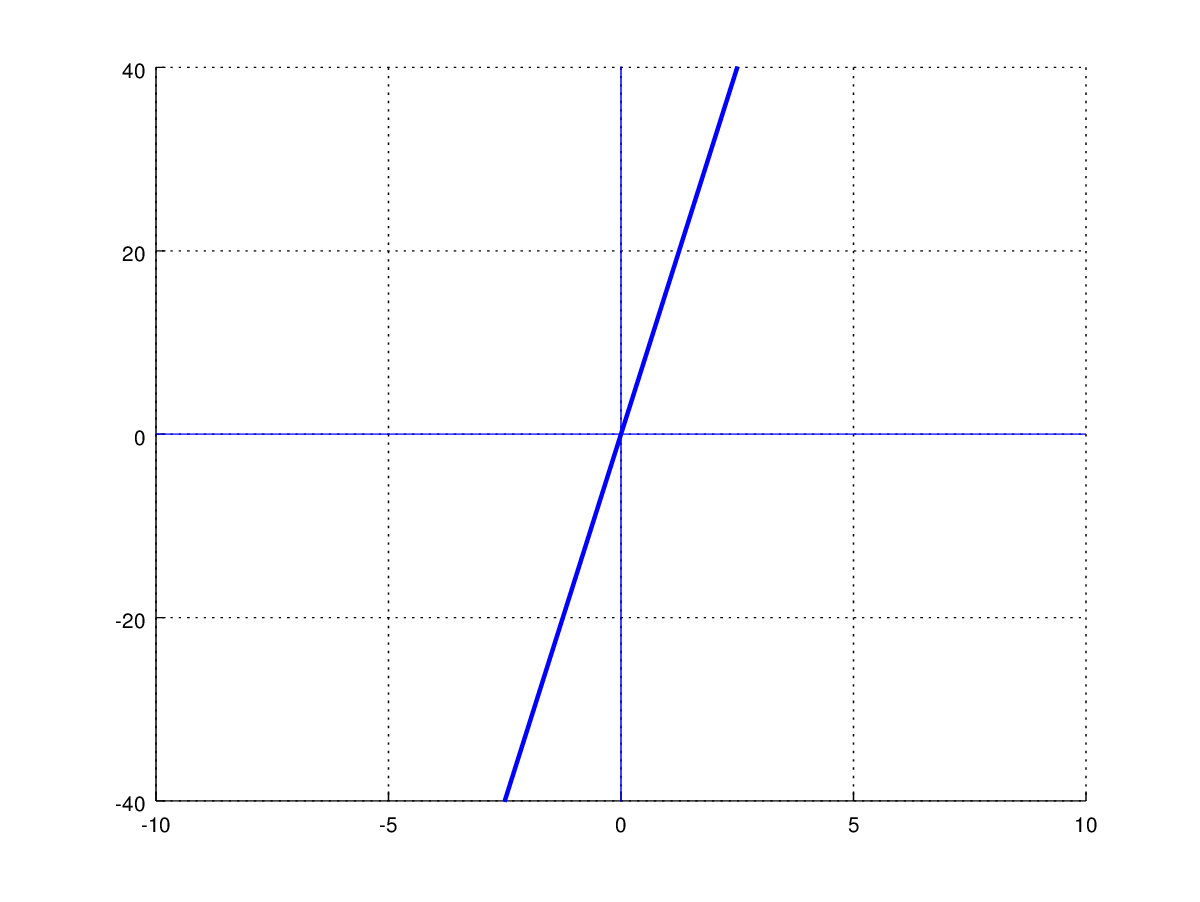
\includegraphics[width=0.9\textwidth]{imgs/ex4c.png}
			\end{figure}
	\end{enumerate}
\end{enumerate}

\end{document}
